\documentclass[a4 paper, 12pt]{article}
\usepackage[utf8]{inputenc}

%% preamble
% preamble.tex

%% packages
% IEEE conference needed
\usepackage{times}
\usepackage{amssymb}
\usepackage{amsmath}
% \usepackage{mathptmx}               % comment for non-IEEE style
\usepackage{graphics}
\usepackage{epsfig}
% others
\usepackage{nicefrac}               % For nice fraction like 1/2
\usepackage{geometry}               % For setting layout
\usepackage{enumitem}               % For customizing items
% For tables
\usepackage{multirow}
\usepackage{makecell}
\usepackage{diagbox}

\usepackage{enumitem}

\usepackage{amsthm}

\usepackage{cite}



%% settings for normal a4 layout
% set indent
% \setlength{\parindent}{0pt}
\setlength{\parskip}{1em}
% set layout
% \geometry{a4paper,scale=0.8}
\geometry{a4paper,left=3cm,right=3cm,top=3cm,bottom=3cm}
% correct bad hyphenation here
\hyphenation{op-tical net-works semi-conduc-tor}


%% new commands
% text
\newcommand{\tn}[1]{\textnormal{#1}}
\newcommand{\tb}[1]{\textbf{#1}}
\newcommand{\ti}[1]{\textit{#1}}
% matrices
\newcommand{\mat}[0]{\begin{bmatrix}}
\newcommand{\mate}[0]{\end{bmatrix}}
% states
\newcommand{\vx}{\mathbf{x}}
\newcommand{\vp}{\mathbf{p}}
\newcommand{\vv}{\mathbf{v}}
\newcommand{\va}{\mathbf{a}}
\newcommand{\vb}{\mathbf{b}}
\newcommand{\vz}{\mathbf{z}}
\newcommand{\vd}{\mathbf{d}}
\newcommand{\vu}{\mathbf{u}}
\newcommand{\vf}{\mathbf{f}}
\newcommand{\vg}{\mathbf{g}}
\newcommand{\vh}{\mathbf{h}}
\newcommand{\vs}{\mathbf{s}}
% sets
\newcommand{\W}{\mathcal{W}}        % Workspace
\newcommand{\X}{\mathcal{X}}        % Configuration space
\newcommand{\Obs}{\mathcal{O}}      % Obstacle regions
\newcommand{\A}{\mathcal{A}}        % Robot occupied space
\newcommand{\U}{\mathcal{U}}        % Control space
\newcommand{\Z}{\mathcal{Z}}        % General decision variables space
\newcommand{\rN}{\mathcal{N}}       % Agent index sets
\newcommand{\oM}{\mathcal{M}}       % Dynamic obstacle index sets
% numbers set
\newcommand{\R}{\mathbb{R}}
\newcommand{\N}{\mathbb{N}}
% operator
\newcommand\norm[1]{\left\|#1\right\|}      % Big norm
\newcommand\abs[1]{\left|#1\right|}         % Big abs
\newcommand\inv[1]{#1^{-1}}                 % Inverse
\newcommand{\atwo}{\mathrm{atan2}}
\newcommand\mc[1]{\mathcal{#1}}
% statistics
\newcommand{\hx}{\hat{\mathbf{x}}}
\newcommand{\hp}{\hat{\mathbf{p}}}
\newcommand{\vsigma}{\mathbf{\sigma}}
\newcommand{\vomega}{\mathbf{\omega}}
\newcommand{\mN}{\mathcal{N}}
\newcommand{\pr}{\textnormal{Pr}}
% symbols
\newcommand{\eps}{\varepsilon}
% other
\newcommand{\ra}{\rightarrow}
\newcommand{\RA}{\Rightarrow}
\newcommand{\half}{\frac{1}{2}}
\newcommand{\quater}{\frac{1}{4}}


%% theorems
\newtheorem{rmk}{\textbf{Remark}}
\newtheorem{thm}{\textbf{Theorem}}
\newtheorem{prop}{\textbf{Proposition}}
\newtheorem{prob}{\textbf{Problem}}
\newtheorem{defi}{\textbf{Definition}}
\newtheorem{algo}{\textbf{Algorithm}}
\newtheorem{cons}{\textbf{Constraint}}


%% title information
\title{
        \Large{DISC Course: Multi-agent Network Dynamics and Games}\\
        \vspace{1em}
        \large\tb{Assignment 2}
}
\author{
        \small Hai Zhu                          \\
        \small Delft University of Technology   \\
        \tt\small h.zhu@tudelft.nl
 }
\date{\small\ti{\today}}

%% document
\begin{document}
%% title
\maketitle


\tb{E2.02 } Determine the convergence rate of the Banach iteration.

\tb{Solution: }
Let $T:\R^n \ra \R^n$ be a $\ell$-contractive mapping ($\ell \in [0,1)$). The Banach iteration approximates a fixed point of $T$ by the following iteration 
\begin{equation}
        x(k+1) = T(x(k))
\end{equation}
Then according to Banach's fixed point theorem, $T$ admits a unique fixed-point $x^\star$, i.e. $x^\star = T(x^\star)$. 

We have proved the Banach's theorem in last assignment. Now we determine the convergence rate of the Banach iteration.

Since $T$ is $\ell$-contraction, we have 
\begin{equation}
        d(T(x), T(y)) \leq \ell d(x,y)
\end{equation}
Thus
\begin{equation}
        \begin{aligned}
                d(x_{n+1},x^\star) &= d(T(x_n),T(x^\star)) \\
                &\leq \ell d(x_n,x^\star)
        \end{aligned}
\end{equation}
and 
\begin{equation}
        \begin{aligned}
                d(x_n,x^\star) &\leq \ell d(x_{n-1},x^\star) \\
                &\leq \ell^2 d(x_{n-2},x^\star) \\ 
                &\leq \dots \\
                &\leq \ell^n d(x_{0},x^\star), \quad n=1,2,\dots
        \end{aligned}
\end{equation}
which determines the rate of convergence of the Banach iteration. Note that $\ell \in [0,1)$ in the above equations. Hence, the convergence rate of the Banach iteration is linear.


% \vspace{2em}
% \tb{E2.03 } Determine the convergence rate of the Krasnoselskii and Mann iteration.

% \tb{Solution: } 
% (a) Let $T: C \ra C$ be a nonexpansive mapping, where the set $C \subset \R^n$ is compact and convex, $\alpha \in (0,1)$. The Krasnoselskij iteration approximates a fixed point of $T$ by the following iteration 
% \begin{equation}
%         x(k+1) = (1-\alpha)x(k) + \alpha T(x(k)),\quad \forall k\in\N
% \end{equation}
% According to Krasnoselskij's theorem, $\exists x^\star \in \tn{fix}(T)$ such that $\lim_{k\ra\infty}x(k) = x^\star$.

% For the mapping $T$, there is 
% \begin{equation}
%         \norm{T(x)-T(y)} \leq \ell \norm{x-y}
% \end{equation}
% where
% \begin{equation}
%         \ell 
%         \begin{cases}
%              \in [0,1), \quad &\tn{$T$ is contractive} \\
%              = 1, \quad &\tn{$T$ is nonexpansive}
%         \end{cases}
% \end{equation}
% Thus, we have
% \begin{equation}
%         \begin{aligned}
%                 \norm{x_{n+1} - x^\star} &= \norm{(1-\alpha)x_n+\alpha T(x_n) - ((1-\alpha)x^\star + \alpha T(x^\star))} \\
%                 &= \norm{(1-\alpha)(x_n-x^\star) + \alpha(T(x_n)-T(x^\star))} \\
%                 &= (1-\alpha)\norm{x_n-x^\star} + \alpha\norm{T(x_n)-T(x^\star)} \\
%                 &\leq (1-\alpha)\norm{x_n-x^\star} + \alpha\ell\norm{x_n-x^\star} \\
%                 &= (1-\alpha+\alpha\ell)\norm{x_n-x^\star}
%         \end{aligned}
% \end{equation}
% and 
% \begin{equation}
%         \begin{aligned}
%                 \norm{x_n - x^\star} &\leq (1-\alpha+\alpha\ell)\norm{x_{n-1}-x^\star} \\
%                 &\leq (1-\alpha+\alpha\ell)^2\norm{x_{n-2}-x^\star} \\
%                 &\leq \dots \\
%                 &\leq (1-\alpha+\alpha\ell)^n\norm{x_0-x^\star}, n = 1, 2, \dots
%         \end{aligned}
% \end{equation}

% We discuss in two cases:
% \begin{itemize}
%         \item Case 1: $\ell \in [0,1)$. Since $\alpha\in(0,1)$ is a given constant, $1-\alpha+\alpha\ell = 1 - \alpha(1-\ell) \in (0,1)$. In this case, the convergence rate of the iteration is linear.

%         \item Case 2: $\ell = 1$. This is use in the definition of the Krasnoselskij iteration where the mapping $T$ is nonexpansive. In this case, $1-\alpha+\alpha\ell = 1$ and thus, $\norm{x_n - x^\star} \leq \norm{x_{n-1} - x^\star} \leq \norm{x_0 - x^\star}$. Hence, the convergence rate of the iteration can be arbitrarily slow.
% \end{itemize}

% (b) The mapping $T: C \ra C$ Lipschitz continuous and strictly pseudo-nonexpansive, where the set $C \subset \R^n$ is compact and convex. The sequence $(\alpha_k)_{k\in\N}$ is positive, bounded and such that $\sum_{k=1}^\infty\alpha_k = \infty$. The Mann iteration approximates a fixed point of $T$ by the following iteration 
% \begin{equation}
%         x(k+1) = (1-\alpha_k)x(k) + \alpha_k T(x(k)),\quad \forall k\in\N
% \end{equation}
% According to the Mann's theorem, $\exists x^\star \in \tn{fix}(T)$ such that $\lim_{k\ra\infty}x(k) = x^\star$.

% It is obvious that when $\alpha_k \equiv \alpha \in (0,1) $, the Mann iteration degenerates to the Krasnoselskii iteration.

% Since $T$ is Lipschitz continuous and strictly pseudo-nonexpansive, we have
% \begin{equation}
%         \norm{T(x)-T(y)} \leq C\norm{x-y}, C\in\R
% \end{equation}
% \begin{equation}
%         \norm{T(x)-T(y)} \leq \norm{x-y} + \kappa\norm{x-T(x)-y+T(y)}, \kappa\in(0,1)
% \end{equation}

% For the Mann iteration, we have
% \begin{equation}
%         \begin{aligned}
%                 \norm{x_{n+1}-x^\star} &= \norm{(1-\alpha_n)x_n+\alpha_nT(x_n)-((1-\alpha^\star)x^\star+\alpha^\star T(x^\star))} \\
%                 &= \norm{(x_n-x^\star) - (\alpha_n x_n - \alpha^\star x^\star) + (\alpha_n T(x_n) - \alpha^\star T(x^\star))}
%         \end{aligned}
% \end{equation}



\vspace{2em}
\tb{E2.06 } Let $A:\R^n \rightrightarrows \R^n$ be a maximally monotone mapping. Show that $\tn{zer}(A+B) = \tn{fix}(\mc{J}_{\gamma A}\circ(\tn{Id}-\gamma B)), \forall \gamma>0$.
\begin{proof}
        
Suppose $x^\star$ is the fixed point, i.e., $x^\star = \mc{J}_{\gamma A}\circ(\tn{Id}-\gamma B)(x^\star)$. Thus
\begin{equation}
        \begin{aligned}
                x^\star = \mc{J}_{\gamma A}\circ(\tn{Id}-\gamma B)(x^\star) 
                &\iff x^\star = (\tn{Id}+\gamma A)^{-1}\circ(\tn{Id}-\gamma B)(x^\star) \\
                &\iff (\tn{Id}+\gamma A)(x^\star) = (\tn{Id}-\gamma B)(x^\star) \\
                &\iff \gamma(A(x^\star)+B(x^\star)) = 0 \\
                &\iff A(x^\star) + B(x^\star) = 0 \\
                &\iff x^\star \in \tn{zer}(A+B)
        \end{aligned}
\end{equation}
Hence, $\tn{zer}(A+B) = \tn{fix}(\mc{J}_{\gamma A}\circ(\tn{Id}-\gamma B)), \forall \gamma>0$.

\end{proof}


\vspace{2em}
\tb{E2.09}

\tb{Solution: }
Since $J_1(x) = x_1x_2$, $J_2(x)= -x_1x_2$ and $\mc{X}_1(\cdot)=\mc{X}_1(\cdot)=\R$, we have 
\begin{equation}
        \tn{proj}_{\mc{X}_1} = \tn{proj}_{\mc{X}_2} = \tn{Id}
\end{equation}
and 
\begin{equation}
        F(x) = \mat \nabla_{x_1} J_1(x_1,x_2)  \\ \nabla_{x_2}J_2(x_1,x_2) \mate = \mat x_2 \\ -x_1 \mate
\end{equation}
According to the forward-backward algorithm
\begin{equation}
        x(k+1) = \tn{proj}_{\Omega}(x(k) - \epsilon F(x(k)))
\end{equation}
we have 
\begin{equation}
        \mat x_1(k+1) \\ x_2(k+1) \mate = \mat x_1(k)-\epsilon(x_2(k)) \\ x_2(k) + \epsilon x_1(k) \mate = \mat 1 &-\epsilon \\ \epsilon &1 \mate \mat x_1(k) \\ x_2(k) \mate
\end{equation}
Denote
\begin{equation}
        T = \mat 1 &-\epsilon \\ \epsilon &1 \mate
\end{equation}
and thus
\begin{equation}
        x(k+1) = T(x(k)) = Tx(k)
\end{equation}
Since $\Lambda(T) = 1\pm \epsilon\tn{i}$. The above mapping is not contractive and thus cannot converge to a fixed point. 

To simulate the iteration, we consider two cases: with constant step size and vanishing step size in the following part. In both two cases, the starting point is chosen to be $x_1(0) = x_2(0) = 1$. The maximum number of iteration is set as $1\times 10^3$. Case (a) is with constant step size $\epsilon = 0.1$ and case (b) is with vanishing step size $\epsilon = \min\{1,\frac{10}{k}\}$. The following two figures show the Simulation results. It can be seen that in both cases, the solution does not converge. 
% Besides, the iteration with constant step size diverges much faster than that with vanishing step size.
% figures
\begin{center}
        \begin{tabular}{c c}
                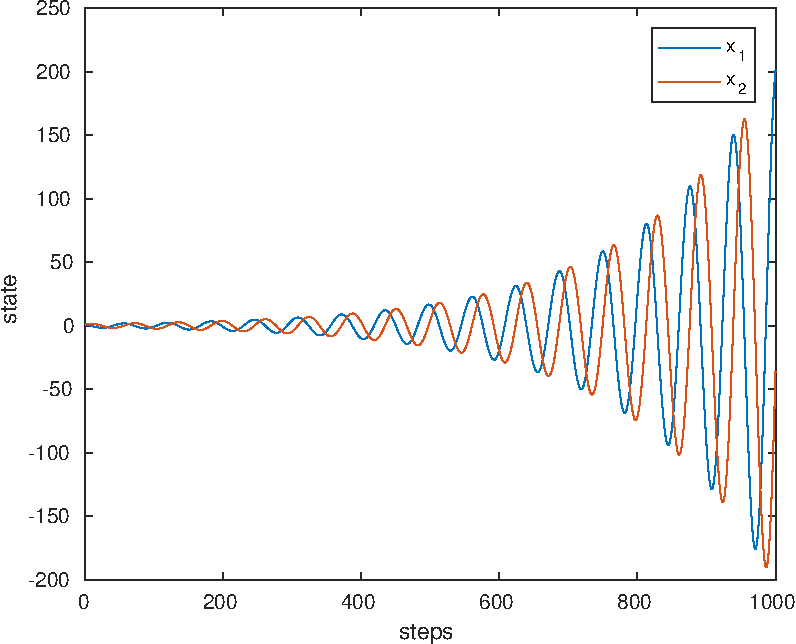
\includegraphics[width=0.45\textwidth]{E209_cons_state.pdf} & 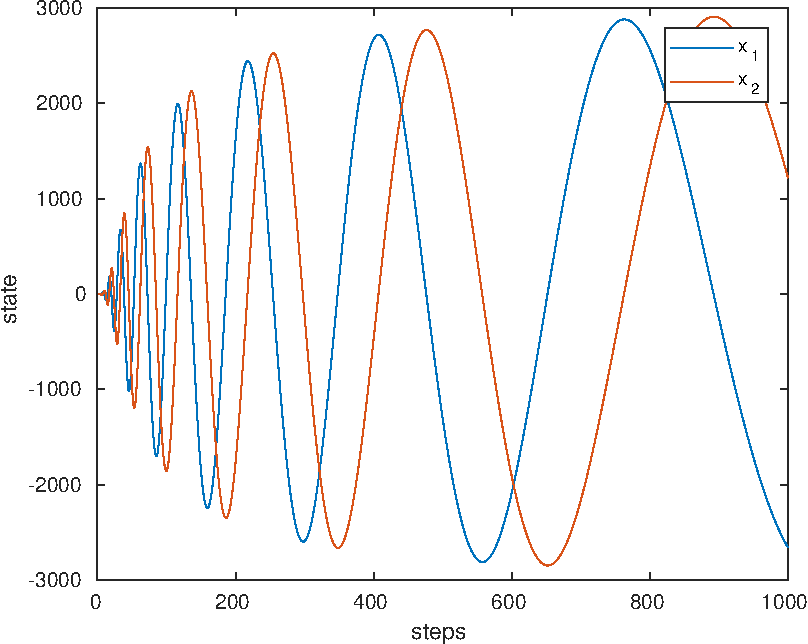
\includegraphics[width=0.45\textwidth]{E209_van_state.pdf} \\
                (a) constant step size $\epsilon=0.1$ & (b) vanishing step size $\epsilon = \min\{1,\frac{10}{k}\}$
        \end{tabular}
\end{center}

\tb{Matlab Code for Simulation}
\lstinputlisting[
  style      = Matlab-editor,
  basicstyle = \mlttfamily,
]{E09.m}



\vspace{2em}
\tb{E2.10 } 

\tb{Solution: }
Since $J_1(x) = \half x_1^2 + x_1x_2$, $J_2(x)= -x_1x_2$ and $\mc{X}_1(\cdot)=\mc{X}_1(\cdot)=\R$, we have 
\begin{equation}
        \tn{proj}_{\mc{X}_1} = \tn{proj}_{\mc{X}_2} = \tn{Id}
\end{equation}
and 
\begin{equation}
        F(x) = \mat \nabla_{x_1} J_1(x_1,x_2)  \\ \nabla_{x_2}J_2(x_1,x_2) \mate = \mat x_1+x_2 \\ -x_1 \mate
\end{equation}
According to the forward-backward algorithm
\begin{equation}
        x(k+1) = \tn{proj}_{\Omega}(x(k) - \epsilon F(x(k)))
\end{equation}
we have 
\begin{equation}
        \mat x_1(k+1) \\ x_2(k+1) \mate = \mat x_1(k)-\epsilon(x_1(k)+x_2(k)) \\ x_2(k) + \epsilon x_1(k) \mate = \mat 1-\epsilon &-\epsilon \\ \epsilon &1 \mate \mat x_1(k) \\ x_2(k) \mate
\end{equation}
Denote
\begin{equation}
        T = \mat 1-\epsilon &-\epsilon \\ \epsilon &1 \mate
\end{equation}
and thus
\begin{equation}
        x(k+1) = T(x(k)) = Tx(k)
\end{equation}
Since $\Lambda(T) = 1 - \frac{\epsilon}{2} \pm \frac{\sqrt{3}}{2}\epsilon \tn{i}$, if we choose $\epsilon \in (0,1)$, then the above iteration becomes the Banach iteration. Hence, it will converge to the fixed point from any starting point. 

To simulate the iteration, we consider two cases: with constant step size and vanishing step size in the following part. In both two cases, the starting point is chosen to be $x_1(0) = x_2(0) = 1$. The tolerance error of iteration is set as $\varepsilon = 1\times10^{-2}$. Case (a) is with constant step size $\epsilon = 0.1$ and case (b) is with vanishing step size $\epsilon = \frac{1}{k}$. The following two figures show the Simulation results. It can be seen that in both cases, the solution converges. Besides, the convergence of the iteration with constant size is faster than that with a vanishing step size.

% figures
\begin{center}
        \begin{tabular}{c c}
                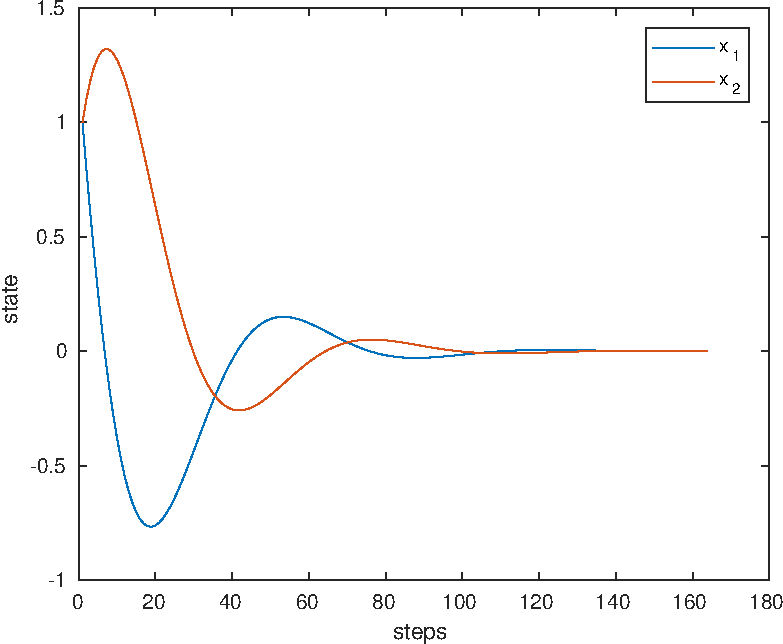
\includegraphics[width=0.45\textwidth]{E210_cons_state.pdf} & 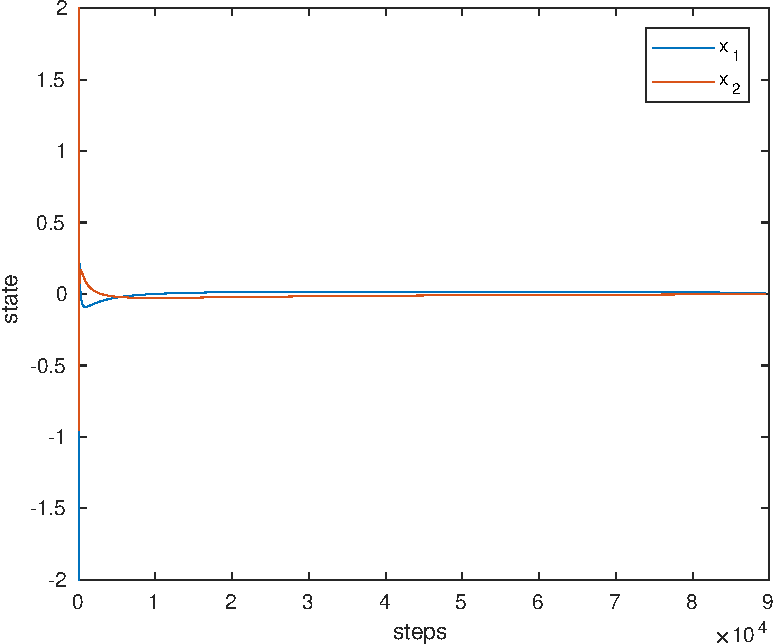
\includegraphics[width=0.45\textwidth]{E210_van_state.pdf} \\
                (a) constant step size $\epsilon=0.1$ & (b) vanishing step size $\epsilon = \frac{1}{k}$
        \end{tabular}
\end{center}

\tb{Matlab Code for Simulation}
\lstinputlisting[
  style      = Matlab-editor,
  basicstyle = \mlttfamily,
]{E10.m}


%% Bibliography
% \bibliographystyle{plainnat}
% \begin{thebibliography}{99}

%         \bibitem{c1} H.K. Khalil. \ti{Nonlinear systems}. Prentice Hall, Upper Saddle River, USA, third edition, 2002.

            
% \end{thebibliography}



\end{document}
